\documentclass{beamer}
\usepackage[utf8]{inputenc}

\usetheme{Madrid}
\usecolortheme{default}
\usepackage{amsmath,amssymb,amsfonts,amsthm}
\usepackage{txfonts}
\usepackage{tkz-euclide}
\usepackage{listings}
\usepackage{adjustbox}
\usepackage{array}
\usepackage{tabularx}
\usepackage{gvv}
\usepackage{lmodern}
\usepackage{circuitikz}
\usepackage{tikz}
\usepackage{graphicx}

\setbeamertemplate{page number in head/foot}[totalframenumber]

\usepackage{tcolorbox}
\tcbuselibrary{minted,breakable,xparse,skins}



\definecolor{bg}{gray}{0.95}
\DeclareTCBListing{mintedbox}{O{}m!O{}}{%
  breakable=true,
  listing engine=minted,
  listing only,
  minted language=#2,
  minted style=default,
  minted options={%
    linenos,
    gobble=0,
    breaklines=true,
    breakafter=,,
    fontsize=\small,
    numbersep=8pt,
    #1},
  boxsep=0pt,
  left skip=0pt,
  right skip=0pt,
  left=25pt,
  right=0pt,
  top=3pt,
  bottom=3pt,
  arc=5pt,
  leftrule=0pt,
  rightrule=0pt,
  bottomrule=2pt,

  colback=bg,
  colframe=orange!70,
  enhanced,
  overlay={%
    \begin{tcbclipinterior}
    \fill[orange!20!white] (frame.south west) rectangle ([xshift=20pt]frame.north west);
    \end{tcbclipinterior}},
  #3,
}
\lstset{
    language=C,
    basicstyle=\ttfamily\small,
    keywordstyle=\color{blue},
    stringstyle=\color{orange},
    commentstyle=\color{green!60!black},
    numbers=left,
    numberstyle=\tiny\color{gray},
    breaklines=true,
    showstringspaces=false,
}
%------------------------------------------------------------
%This block of code defines the information to appear in the
%Title page
\title %optional
{3.3.15}
\date{\today}
%\subtitle{A short story}

\author % (optional)
{Shivam Sawarkar \\ AI25BTECH11031}



\begin{document}


\frame{\titlepage}
\begin{frame}{Question}
    Find the equation of the set of points $P$ the sum of whose distances from $A(4, 0, 0)$ and $B(-4, 0, 0)$ is equal to 10.
\end{frame}

\begin{frame}{Solution}
    We want the locus of points $\vec{p} \in \mathbb{R}^3$ such that
\begin{align}
\norm{\vec{p}-\vec{A}}+\norm{\vec{p}-\vec{B}} = 10,
\end{align}
where
\begin{align}
\vec{A} = \myvec{4 \\ 0 \\ 0}, \quad
\vec{B} = \myvec{-4 \\ 0 \\ 0}.
\end{align}

\textbf{Step 1 - Decomposition of $\vec{p}$:}

Define the unit vector along the foci axis:
\begin{align}
\vec{e} = \frac{\vec{A} - \vec{B}}{\norm{\vec{A}-\vec{B}}}
= \frac{\myvec{8 \\ 0 \\ 0}}{8} = \myvec{1 \\ 0 \\ 0}.
\end{align}
\end{frame}

\begin{frame}{Solution}
    Decompose $\vec{p}$ into parallel and perpendicular components:
\begin{align}
\vec{p} = (\vec{e}^\top \vec{p})\,\vec{e}
+ \big( I - \vec{e}\vec{e}^\top \big) \vec{p}.
\end{align}

Let:
\begin{align}
\alpha := \vec{e}^\top \vec{p}, \quad
R := I - \vec{e}\vec{e}^\top.
\end{align}
Then the perpendicular squared component is:
\begin{align}
s := \|R\vec{p}\|^2.
\end{align}

\textbf{Step 2 - Distances to the foci:}

\begin{align}
\norm{\vec{p}-\vec{A}}
= \sqrt{(\alpha - 4)^2 + s}, \quad
\norm{\vec{p}-\vec{B}}
= \sqrt{(\alpha + 4)^2 + s}.
\end{align}

The condition becomes:
\begin{align}
\sqrt{(\alpha - 4)^2 + s} + \sqrt{(\alpha + 4)^2 + s} = 10.
\end{align}
\end{frame}

\begin{frame}{Solution}
    \textbf{Step 3 - Eliminate square roots:}

Square both sides and rearrange to eliminate the radicals.
After algebraic manipulation, we obtain:
\begin{align}
-36\,\alpha^2 - 100\,s + 900 = 0.
\end{align}

The equation becomes:
\begin{align}
-36\,\vec{p}^\top (\vec{e}\vec{e}^\top) \vec{p}
- 100\,\vec{p}^\top R \vec{p}
+ 900 = 0.
\end{align}

\begin{align}
\vec{p}^\top\left(
-36\,\vec{e}\vec{e}^\top - 100\,R
\right)\vec{p} + 900 = 0.
\end{align}
\end{frame}

\begin{frame}{Solution}
    \textbf{Step 4 - Simplify using $R = I - \vec{e}\vec{e}^\top$:}
\begin{align}
-36\,\vec{e}\vec{e}^\top - 100(I - \vec{e}\vec{e}^\top)
= -100I + 64\,\vec{e}\vec{e}^\top.
\end{align}

Thus:
\begin{align}
\vec{p}^\top\left(
I - \frac{64}{100}\vec{e}\vec{e}^\top
\right)\vec{p} = 9.
\end{align}

\begin{align}
\boxed{
\vec{p}^\top
\myvec{
\tfrac{1}{25} & 0 & 0 \\ 
0 & \tfrac{1}{9} & 0 \\ 
0 & 0 & \tfrac{1}{9}
}
\vec{p} = 1,
}
\end{align}
which is the equation of a prolate spheroid with semi-axes $5,3,3$.
\end{frame}

\begin{frame}{Plot}
    \begin{figure}
        \centering
        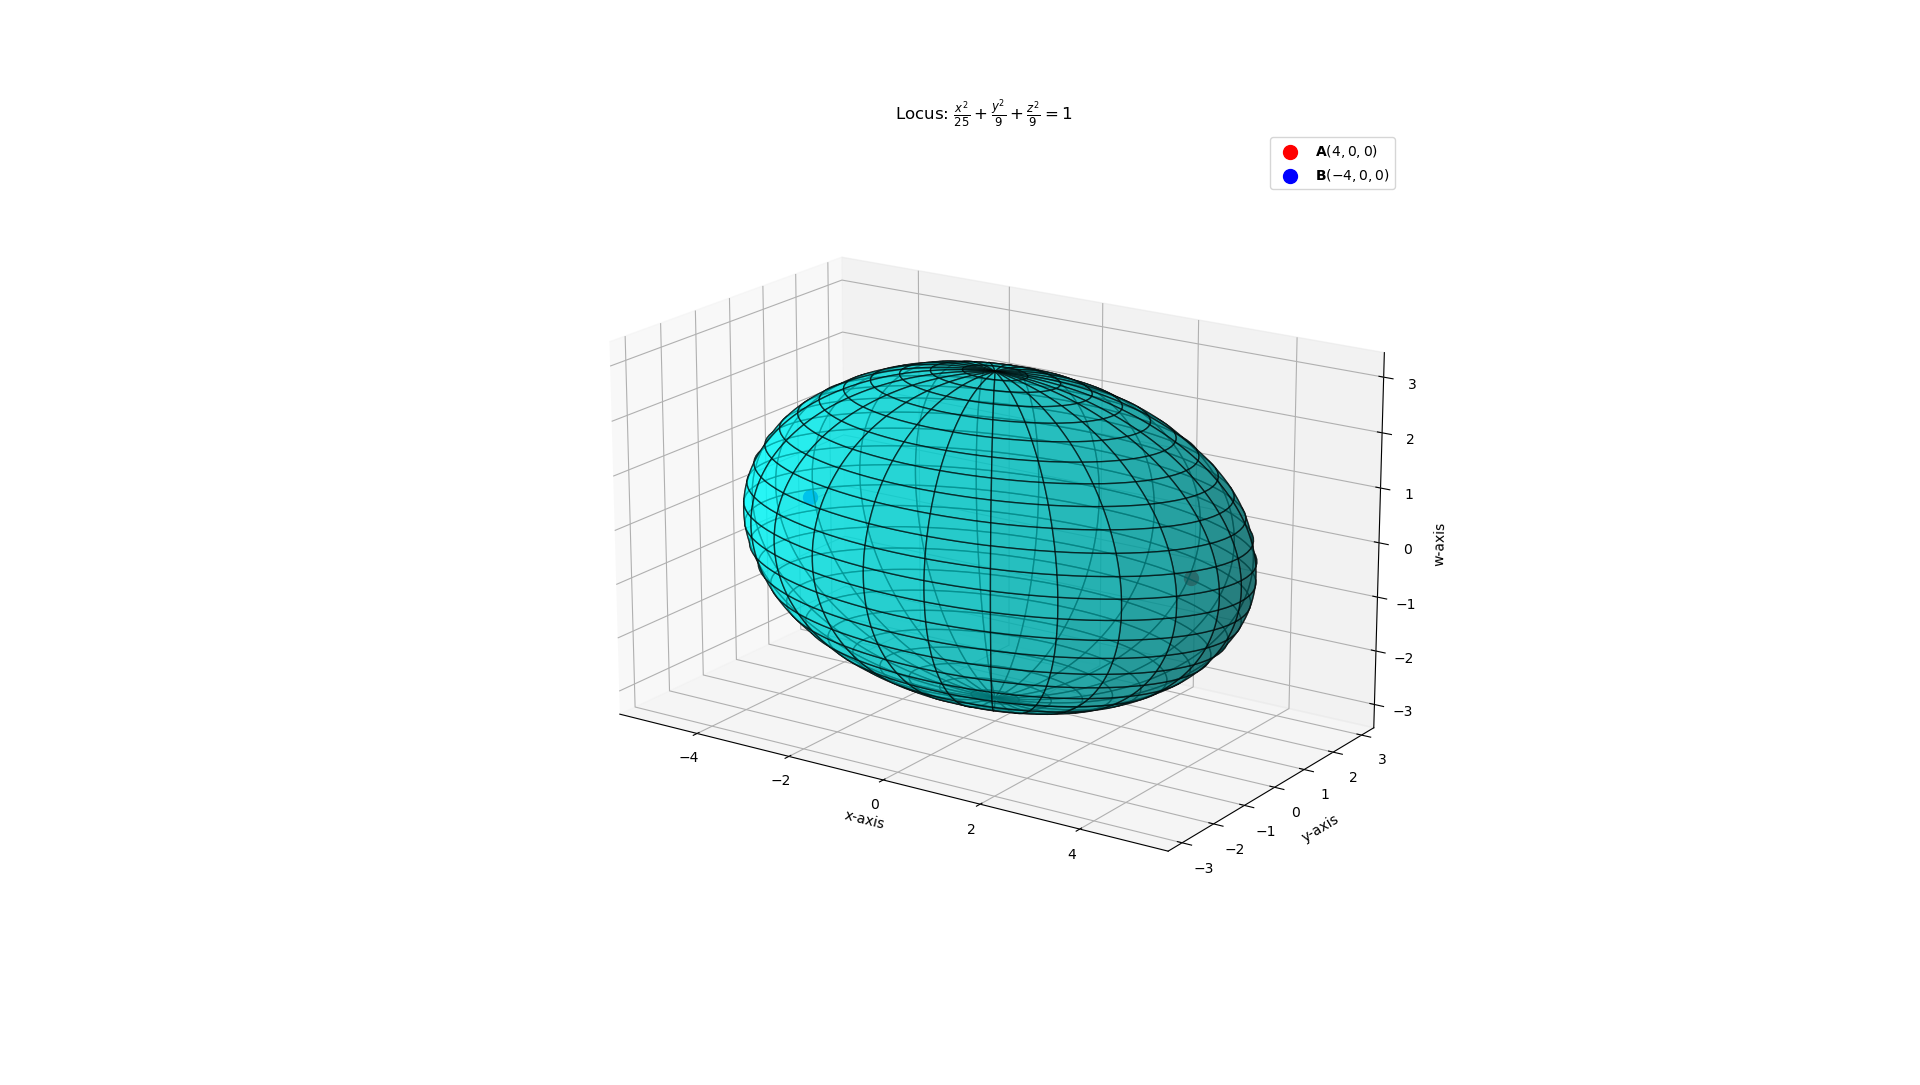
\includegraphics[width=1\linewidth]{figs/plot9.png}
        \caption{}
        \label{fig:placeholder}
    \end{figure}
\end{frame}

\begin{frame}[fragile]{C Code}
    \begin{verbatim}
#ifndef LOCUS_H
#define LOCUS_H

#include <stdio.h>
#include <math.h>

void standard_form(double A[3], double B[3], double constant_sum,
                   double *a2, double *b2, double *c2) {
    double dist_AB = sqrt(pow(A[0]-B[0],2) + pow(A[1]-B[1],2) + pow(A[2]-B[2],2));
    double a = constant_sum / 2.0;
    double c = dist_AB / 2.0;
    double b = sqrt(a*a - c*c);
    *a2 = a*a;
    *b2 = b*b;
    *c2 = b*b; // spheroid symmetry
}
#endif
    \end{verbatim}
\end{frame}

\begin{frame}[fragile]{C Code}
    \begin{verbatim}
#include <stdio.h>
#include <math.h>
#include "solution.h"

int main() {
    double A[3], B[3];
    double constant_sum;
    double a2, b2, c2;

    printf("Enter coordinates of point A (Ax Ay Az): ");
    scanf("%lf %lf %lf", &A[0], &A[1], &A[2]);

    printf("Enter coordinates of point B (Bx By Bz): ");
    scanf("%lf %lf %lf", &B[0], &B[1], &B[2]);
    \end{verbatim}
\end{frame}

\begin{frame}[fragile]{C Code}
    \begin{verbatim}
    printf("Enter the constant sum of distances: ");
    scanf("%lf", &constant_sum);

    standard_form(A, B, constant_sum, &a2, &b2, &c2);

    printf("\nStandard form of the locus equation:\n");
    printf("x^2/(%.6lf) + y^2/(%.6lf) + z^2/(%.6lf) = 1\n", a2, b2, c2);

    printf("\nWhere:\n");
    printf("a = %.6lf, b = %.6lf, c = %.6lf\n", sqrt(a2), sqrt(b2), sqrt(c2));

    return 0;
}
    \end{verbatim}
\end{frame}

\begin{frame}[fragile]{Python Code}
    \begin{verbatim}
import numpy as np

def standard_form(A, B, constant_sum):
    # Distance between foci
    dist_AB = np.linalg.norm(np.array(A) - np.array(B))
    
    # Semi-major axis
    a = constant_sum / 2.0
    # Focal length
    c = dist_AB / 2.0
    # Semi-minor axis
    b = np.sqrt(a*a - c*c)

    return a*a, b*b, b*b  # a², b², c²
    \end{verbatim}
\end{frame}

\begin{frame}[fragile]{Python Code}
    \begin{verbatim}
if __name__ == "__main__":
    A = list(map(float, input("Enter coordinates of point A (Ax Ay Az): ").split()))
    B = list(map(float, input("Enter coordinates of point B (Bx By Bz): ").split()))
    constant_sum = float(input("Enter the constant sum of distances: "))

    a2, b2, c2 = standard_form(A, B, constant_sum)

    print("\nStandard form of the locus equation:")
    print(f"x^2/({a2:.6f}) + y^2/({b2:.6f}) + z^2/({c2:.6f}) = 1")
    print("\nWhere:")
    print(f"a = {np.sqrt(a2):.6f}, b = {np.sqrt(b2):.6f}, c = {np.sqrt(c2):.6f}")
    \end{verbatim}
\end{frame}

\begin{frame}[fragile]{Python + C Code}
    \begin{verbatim}
import ctypes
import numpy as np

# Load the shared library
locus = ctypes.CDLL("./solution.so")

# Define argument types
locus.standard_form.argtypes = [
    ctypes.POINTER(ctypes.c_double), ctypes.POINTER(ctypes.c_
    double),
    ctypes.c_double,
    ctypes.POINTER(ctypes.c_double), ctypes.POINTER(ctypes.c_
    double), ctypes.POINTER(ctypes.c_double)
]
    \end{verbatim}
\end{frame}

\begin{frame}[fragile]{Python + C Code}
    \begin{verbatim}
def standard_form(A, B, constant_sum):
    A_arr = (ctypes.c_double * 3)(*A)
    B_arr = (ctypes.c_double * 3)(*B)
    a2 = ctypes.c_double()
    b2 = ctypes.c_double()
    c2 = ctypes.c_double()
    locus.standard_form(A_arr, B_arr, constant_sum, 
    ctypes.byref(a2), ctypes.byref(b2), ctypes.byref(c2))
    return a2.value, b2.value, c2.value

if __name__ == "__main__":
    A = list(map(float, input("Enter coordinates of point 
    A (Ax Ay Az): ").split()))
    B = list(map(float, input("Enter coordinates of point 
    B (Bx By Bz): ").split()))
    constant_sum = float(input("Enter the constant sum of 
    distances: "))
    \end{verbatim}
\end{frame}

\begin{frame}[fragile]{Python + C Code}
    \begin{verbatim}
    a2, b2, c2 = standard_form(A, B, constant_sum)
    print("\nStandard form of the locus equation:")
    print(f"x^2/({a2:.6f}) + y^2/({b2:.6f}) + z^2/({c2:.6f})
    = 1")
    print("\nWhere:")
    print(f"a = {np.sqrt(a2):.6f}, b = {np.sqrt(b2):.6f}, 
    c = {np.sqrt(c2):.6f}")
    \end{verbatim}
\end{frame}




\end{document}